\documentclass[12pt, oneside]{article} 
\usepackage{amsmath, amsthm, amssymb, calrsfs, wasysym, verbatim, bbm, color, graphics, geometry, setspace, listings}
\usepackage{graphicx}
\usepackage[utf8]{inputenc}
\setlength{\parindent}{4em}
\usepackage[dvipsnames]{xcolor}
\usepackage{setspace}
\onehalfspacing
\usepackage{mathrsfs}
\usepackage{fancyhdr}
\usepackage{caption}
\usepackage{subcaption}
\usepackage{multirow}
\usepackage{tabu}
\newsavebox\mybox
\usepackage[shortlabels]{enumitem}
\usepackage[normalem]{ulem}
\usepackage{mathtools}
\usepackage[normalem]{ulem} 
\newtheorem{algo}{Algorithm}


\begin{document}

\section{Mathematical Formulation}
\subsection{Notations}
Before we state our problem, let us first define the notations used in the study. Our first-stage decision variable is binary such that,
\begin{align*}
    z_e =
    \begin{cases}
      1, & \text{if arc \textit{e} is used} \\
      0, & \text{otherwise}
    \end{cases}
\end{align*}
Our second stage decision variable $x_e^s$ is the flow on arc \textit{e} in scenario $s$.

Deterministic data are defined below:
\begin{align*}
    s \ \ \ \ \ \ & \text{scenario,} \ \ \ \  \forall s = 1,...,S \\ 
    f_e \ \ \ \ \ \ & \text{fixed charge for using arc} \ e \\
    c_e \ \ \ \ \ \ & \text{cost of shipping one unit using arc} \ e \\
    d \ \ \ \ \ \ & \text{demand}  \\
    p_s \ \ \ \ \ \ & \text{probability}
\shortintertext{%
\hspace{1.55cm}  Random data used in the models are defined below:%
}
    u_e^s \ \ \ \ \ \ & \text{full capacity of arc} \ e \\
    y_e^s \ \ \ \ \ \ & \text{unmet demand at arc} \ e \\
    \sigma_e^s \ \ \ \ \ \ & \text{cost of shortfall}
\end{align*}

\subsection{Problem Statement}
\begin{center}
    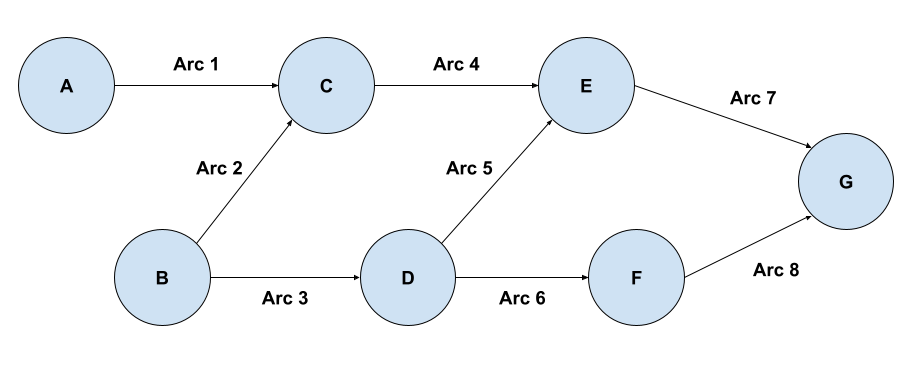
\includegraphics[width=0.9\linewidth]{model.png}
\end{center}

In our network model (shown above), node A and B are supply nodes, node C, D, E, F are transshipment nodes, and node G is a demand node. Now we will define our linear program,
\begin{equation*}
\begin{array}{ll@{}ll}
    \min_{x,y,z}      &   \sum_{e=1}^8 f_e z_e + \sum_{s=1}^S \bigg( \sum_{e=1}^8 p_s x_e^s c_e + p_s y_e^s \sigma_e^s \bigg) \\
    \text{subject to} &   z_e \in  \{0,1\},\ \ \ \ \ \ \ \ \ \ \ \ \ \ e=1 ,\dots, 8 \\
                      & 0  \le x_e^s  \le u_e^sz_e \ \ \ \ \ \ \ \ \ \  \forall s = 1,...,S \\
                      & \sum_{e=1}^8 x_e^s  \ge d- y_e^s \\
                      & x_7^s + x_8^s = d- y_e^s \\
                      & x_1^s + x_2^s = x_4^s \\
                      & x_5^s + x_6^s = x_5^s \\
                      & x_4^s + x_5^s = x_7^s \\
                      & x_6^s         = x_8^s
\end{array}
\end{equation*}
We first have the constraint on our first-stage binary variable defined earlier. We also want the flow on arc $e$ in scenario $s$ to be nonnegative, but less than or equal to the full capacity of arc $e$, if used, i.e. 
$$0 \le x_e^s \le u_e^sz_e \ \ \forall s = 1,...,S$$ The sum of all flows on arc $e$ in each scenario $s$ must be greater than or equal to the difference in demand and the shortfall, i.e. $$\sum_{e \ \text{into destination}} x_e^s \ge d-y_e^s$$ The equality constraints represent the flow conservation for each $s$.

\end{document}
